\documentclass[aspectratio=169, lualatex, handout]{beamer}
\makeatletter\def\input@path{{theme/}}\makeatother\usetheme{cipher}

\title{Applied Cryptography}
\author{Nadim Kobeissi}
\institute{American University of Beirut}
\instituteimage{images/aub_white.png}
\date{\today}
\coversubtitle{CMPS 297AD/396AI\\Fall 2025}
\coverpartname{Part 2: Real-World Cryptography}
\covertopicname{2.8: Zero-Knowledge Proofs}
\coverwebsite{https://appliedcryptography.page}

\begin{document}
\begin{frame}[plain]
	\titlepage
\end{frame}

% zkSNARKs, arithmetization
% Sigma, Fiat-Shamir
% That recent paper about limitations of Fiat-Shamir
% OPAQUE, since it was mentioned 100 times in earlier topics
% SRP? Socialist Millionaire? Or too basic?
% Much more, TBD
%
% Use cases:
% - Zcash
% - Penumbra

\incompleteslideswarning

\section{Introduction}

\incompleteslideswarning

\begin{frame}{Zero-knowledge proofs: magic, but real}
	\begin{columns}[c]
		\begin{column}{0.5\textwidth}
			\textbf{Imagine this scenario:}
			\begin{itemize}
				\item I claim to know the password to a secret vault
				\item You need to verify I really know it
				\item But I don't want to tell you the password!
			\end{itemize}
			\vspace{0.5em}
			\textbf{Seems impossible?}
			\begin{itemize}
				\item How can I prove knowledge without revealing it?
				\item This is the magic of zero-knowledge proofs
			\end{itemize}
		\end{column}
		\begin{column}{0.5\textwidth}
			\begin{block}{Zero-knowledge property}
				A proof that reveals \textbf{nothing} except the truth of the statement being proven
			\end{block}
			\vspace{0.5em}
			\begin{alertblock}{The paradox}
				Convince you completely while teaching you nothing
			\end{alertblock}
		\end{column}
	\end{columns}
\end{frame}

\begin{frame}{What makes zero-knowledge proofs special?}
	\textbf{Traditional proof:}
	\begin{itemize}
		\item ``Here's my password: \texttt{hunter2}''
		\item You learn the secret itself
		\item You could now impersonate me
	\end{itemize}
	\vspace{1em}
	\textbf{Zero-Knowledge proof:}
	\begin{itemize}
		\item ``I'll convince you I know the password''
		\item You learn \textit{only} that I know it
		\item You gain no ability to prove it yourself
		\item You can't replay my proof to others
	\end{itemize}
\end{frame}

\begin{frame}{The three zero-knowledge properties}
	\begin{block}{1. Completeness}
		If the statement is true, an honest prover can convince an honest verifier
	\end{block}
	\begin{block}{2. Soundness}
		If the statement is false, no cheating prover can convince an honest verifier (except with negligible probability)
	\end{block}
	\begin{block}{3. Zero-Knowledge}
		The verifier learns nothing beyond the validity of the statement
	\end{block}
	\vspace{0.25em}
	\begin{center}
		\textbf{These three properties together create the ``magic''}
	\end{center}
\end{frame}

\begin{frame}{Example: Proving Knowledge of a Private Key}
	\begin{columns}[c]
		\begin{column}{0.5\textwidth}
			\textbf{The Setup:}
			\begin{itemize}
				\item Public key: $A = g^{a}$
				\item I claim to know $a$
				\item But revealing $a$ would compromise security
			\end{itemize}
			\vspace{0.5em}
			\textbf{Zero-Knowledge Solution:}
			\begin{enumerate}
				\item Interactive protocol
				\item Multiple rounds of challenges
				\item Statistically convincing
				\item Reveals nothing about $a$
			\end{enumerate}
		\end{column}
		\begin{column}{0.5\textwidth}
			\begin{alertblock}{Can't prove to others}
				After our interaction:
				\begin{itemize}
					\item You're 100\% convinced I know $a$
					\item You've learned nothing about $a$
					\item You can't prove to others that I know it
				\end{itemize}
			\end{alertblock}
			\vspace{0.5em}
			\begin{exampleblock}{No ``trace'' or ``evidence''}
				The interaction leaves no transferable evidence
			\end{exampleblock}
		\end{column}
	\end{columns}
\end{frame}

\begin{frame}{Schnorr Identification Protocol}
	\vspace{-1.5cm}
	\begin{center}\resizebox{0.8\textwidth}{!}{
			\begin{msc}{}
				\setmscvalues{small}
				\drawframe{none}
				\setlength{\instdist}{8cm}
				\setlength{\instwidth}{2cm}
				\declinst{prover}{}{Prover}
				\declinst{verifier}{}{Verifier}
				\action*{$\begin{array}{l}
							\text{Knows generator}~g         \\
							\text{Knows prime}~n             \\
							\text{Knows secret}~a            \\
							y \twoheadleftarrow \mathbb{Z}_n \\
							Y = g^y
						\end{array}$}{prover}
				\action*{$\begin{array}{l}
							\text{Knows generator}~g                 \\
							\text{Knows prime}~n                     \\
							\text{Knows prover's public key}~A = g^a \\
						\end{array}$}{verifier}
				\nextlevel[7]
				\mess{$Y$}{prover}{verifier}
				\nextlevel[1]
				\action*{$c \twoheadleftarrow \mathbb{Z}_n$}{verifier}
				\nextlevel[2]
				\mess{$c$}{verifier}{prover}
				\nextlevel[1]
				\action*{$r = (y + ca) \bmod n$}{prover}
				\nextlevel[2]
				\mess{$r$}{prover}{verifier}
				\nextlevel[1]
				\action*{$g^r \overset{?}{\equiv} Y \cdot A^c$}{verifier}
				\nextlevel[2]
			\end{msc}
		}\end{center}
\end{frame}

\begin{frame}{Schnorr Identification Protocol}
	\begin{columns}[c]
		\begin{column}{0.6\textwidth}
			\begin{itemize}
				\item \textbf{Interactive proof:} Multiple rounds of communication
				\item \textbf{Commitment phase:} Prover commits to random $Y = g^y$
				\item \textbf{Challenge phase:} Verifier sends random challenge $c$
				\item \textbf{Response phase:} Prover computes $r = y + ca$
				\item \textbf{Verification:} Check if $g^r = Y \cdot A^c$
				\item \textbf{Zero-knowledge property:} $r$ reveals nothing about $a$ due to random masking by $y$
				\item \textbf{Soundness:} Without knowing $a$, prover can't answer random challenges correctly
			\end{itemize}
		\end{column}
		\begin{column}{0.4\textwidth}
			\vspace{-1.5cm}
			\begin{center}\resizebox{1\textwidth}{!}{
					\begin{msc}{}
						\setmscvalues{small}
						\drawframe{none}
						\setlength{\instdist}{8cm}
						\setlength{\instwidth}{2cm}
						\declinst{prover}{}{Prover}
						\declinst{verifier}{}{Verifier}
						\action*{$\begin{array}{l}
									\text{Knows generator}~g         \\
									\text{Knows prime}~n             \\
									\text{Knows secret}~a            \\
									y \twoheadleftarrow \mathbb{Z}_n \\
									Y = g^y
								\end{array}$}{prover}
						\action*{$\begin{array}{l}
									\text{Knows generator}~g                 \\
									\text{Knows prime}~n                     \\
									\text{Knows prover's public key}~A = g^a \\
								\end{array}$}{verifier}
						\nextlevel[7]
						\mess{$Y$}{prover}{verifier}
						\nextlevel[1]
						\action*{$c \twoheadleftarrow \mathbb{Z}_n$}{verifier}
						\nextlevel[2]
						\mess{$c$}{verifier}{prover}
						\nextlevel[1]
						\action*{$r = (y + ca) \bmod n$}{prover}
						\nextlevel[2]
						\mess{$r$}{prover}{verifier}
						\nextlevel[1]
						\action*{$g^r \overset{?}{\equiv} Y \cdot A^c$}{verifier}
						\nextlevel[2]
					\end{msc}
				}\end{center}
		\end{column}
	\end{columns}
\end{frame}

\begin{frame}{The verifier learned literally nothing new}
	\begin{columns}[c]
		\begin{column}{0.55\textwidth}
			\begin{itemize}
				\item After the protocol, you're convinced I know the secret
				\item But you can't convince anyone else!
				\item Why? The transcript looks identical to \textbf{something you could have generated alone}
				\item \textbf{The simulation argument:}
				      \begin{itemize}
					      \item You could have picked $r$ and $c$ randomly
					      \item Then computed $Y = g^r / A^c$
					      \item This produces a valid-looking transcript!
					      \item No way to distinguish from real interaction
				      \end{itemize}
			\end{itemize}
		\end{column}
		\begin{column}{0.45\textwidth}
			\resizebox{0.8\textwidth}{!}{%
				\begin{minipage}{\textwidth}
					\begin{alertblock}{Self-generated transcripts}
						For any challenge $c$ and response $r$:
						\begin{itemize}
							\item Set $Y = g^r / A^c$
							\item Now $(Y, c, r)$ is a valid transcript
							\item Indistinguishable from real protocol
							\item Real interaction: Prover knows secret
							\item Simulated transcript: No secret needed
							\item Both look exactly the same!
							\item This is what makes it ``zero-knowledge''
						\end{itemize}
					\end{alertblock}
				\end{minipage}%
			}
		\end{column}
	\end{columns}
\end{frame}

\begin{frame}{In other words...}
	\begin{center}
		\sslinked{
			\sslibrary{}{schnorr-real}{
				\sslibrarysubroutine{schnorr.transcript}{a}{
					$A := g^a$ \\
					$y \twoheadleftarrow \mathbb{Z}_n$ \\
					$Y := g^y$ \\
					$c \twoheadleftarrow \mathbb{Z}_n$ \\
					$r := (y + ca) \bmod n$ \\
					return $(A, Y, c, r)$
				}{1}
			}{1}
		}{\interchangeable}{
			\sslibrary{}{schnorr-fake}{
				\sslibrarysubroutine{schnorr.transcript}{a}{
					$A := g^a$ \\
					$c \twoheadleftarrow \mathbb{Z}_n$ \\
					$r \twoheadleftarrow \mathbb{Z}_n$ \\
					$Y := g^r \cdot (A^c)^{-1}$ \\
					return $(A, Y, c, r)$
				}{1}
			}{1}
		}
	\end{center}
\end{frame}

\begin{frame}{A parable}
	\begin{center}
		\vfill
		\large
		\textit{\rmfamily ``King Richard decides to hold an archery competition to identify the best archer in the land. He constructs a long wooden wall, with many targets painted on it. During the competition, he is stunned as Robin Hood stands 100 meters away from the wall and fires one arrow into the center of each of the targets. Of course, Robin Hood is declared the winner.''}
		\vfill
	\end{center}
\end{frame}

\begin{frame}{A parable}
	\begin{center}
		\vfill
		\large
		\textit{\rmfamily ``Later that day, the Sheriff of Nottingham arrives at the King's castle. The King describes Robin Hood's exceptional performance, pointing to the arrows still in the targets. The Sheriff is not impressed. “Robin Hood is a fraud and a liar. Those arrows prove nothing,” he says. He takes his own bow and fires a series of arrows into blank parts of the wall. He finds a bucket of paint and paints a target around each of his arrows. ``See,'' he says again, ``arrows in targets prove nothing!''''}
		\vfill
	\end{center}
\end{frame}

\begin{frame}{Another parable}
	\begin{center}
		\vfill
		\large
		\textit{\rmfamily ``Alice, whose public key is $A = g^a$, contacts Bob and uses Schnorr's protocol to prove that she knows the secret key $a$. Bob is convinced that he is talking to Alice, and he writes down everything he sees: $(A, Y, c, r)$.''}
		\vfill
	\end{center}
\end{frame}

\begin{frame}{Another parable}
	\begin{center}
		\vfill
		\large
		\textit{\rmfamily ``Later that day, Charlie arrives at Bob's house. Bob mentions that he talked to Alice earlier in the day, and he shows Charlie the accepting transcript $(A,Y,c,r)$. ``That proves nothing,'' says Charlie, and he proceeds to generate his own accepting transcript $(A,Y',c',r')$, even though he doesn't know $a$.''}
		\vfill
	\end{center}
\end{frame}

\begin{frame}{ZK can scale to entire systems}{Reminder}
	\begin{columns}[c]
		\begin{column}{0.6\textwidth}
			\begin{itemize}[<+->]
				\item As seen previously, you can build entire \textbf{zero-knowledge protocols}, not just primitives that prove knowledge of certain numbers.
				\item ``Zero-knowledge virtual machines'' where you can execute
				      an entire program that runs as a zero-knowledge proof.
				\item ZKP battleship game: server proves to the players that its
				      output to their battleship guesses is correct, without revealing any
				      additional information (e.g. ship location).
			\end{itemize}
		\end{column}
		\begin{column}{0.4\textwidth}
			\imagewithcaption{battleship.jpg}{Battleship board game. Source: Hasbro}
		\end{column}
	\end{columns}
\end{frame}

\begin{frame}{Beyond authentication: the power of zero-knowledge}
	\begin{center}
		\textbf{Zero-knowledge is not limited to proving identity!}
	\end{center}
	\vspace{0.25em}
	\begin{columns}[c]
		\begin{column}{0.6\textwidth}
			\begin{itemize}
				\item \textbf{Can prove statements like:}
				      \begin{itemize}
					      \item \textit{``I know a solution to this Sudoku puzzle''}
					      \item \textit{``This encrypted value is in range [0, 100]''} (range proofs)
					      \item \textit{``I performed this computation correctly''}
					      \item \ldots without revealing any information!
				      \end{itemize}
			\end{itemize}
		\end{column}
		\begin{column}{0.4\textwidth}
			\begin{itemize}
				\item \textbf{Applications:}
				      \begin{itemize}
					      \item Private transactions (Zcash)
					      \item Anonymous credentials
					      \item Secure voting systems
					      \item Privacy-preserving audits
				      \end{itemize}
			\end{itemize}
		\end{column}
	\end{columns}
\end{frame}

\incompleteslideswarning

\section{Sigma Protocols}

\begin{frame}{From Schnorr to Sigma, a general framework}
	\begin{columns}[c]
		\begin{column}{0.5\textwidth}
			\textbf{Schnorr was just the beginning!}
			\begin{itemize}
				\item Schnorr proves: ``I know $a$ such that $g^a = A$''
				\item What if we want to prove other statements?
				\item Enter \textbf{Sigma protocols}: a general framework
			\end{itemize}
			\vspace{0.5em}
			\textbf{The pattern:}
			\begin{itemize}
				\item Public instance: $X$
				\item Private witness: $W$
				\item Relation: $R(X, W) = \text{true}$
			\end{itemize}
		\end{column}
		\begin{column}{0.5\textwidth}
			\begin{exampleblock}{Examples of relations}
				\begin{itemize}
					\item ``I know $a$ such that $g^a = X$''
					\item ``I know $(r, s)$ such that $g^r h^s = X$''
					\item ``I know a factorization of $X$''
					\item ``I know a graph coloring for $X$''
				\end{itemize}
			\end{exampleblock}
		\end{column}
	\end{columns}
\end{frame}

\begin{frame}{Sigma protocol structure}
	\vspace{-1.5cm}
	\begin{center}\resizebox{0.8\textwidth}{!}{
			\begin{msc}{}
				\setmscvalues{small}
				\drawframe{none}
				\setlength{\instdist}{8cm}
				\setlength{\instwidth}{2cm}
				\declinst{prover}{}{Prover}
				\declinst{verifier}{}{Verifier}
				\action*{$\begin{array}{l}
							\text{Knows instance}~X                \\
							\text{Knows witness}~W                 \\
							\text{Such that}~R(X, W) = \text{true} \\
						\end{array}$}{prover}
				\action*{$\begin{array}{l}
							\text{Knows instance}~X \\
						\end{array}$}{verifier}
				\nextlevel[4]
				\action*{$(Y, \sigma) \leftarrow \text{Commit}(X, W)$}{prover}
				\nextlevel[2]
				\mess{$Y$ (commitment)}{prover}{verifier}
				\nextlevel[1]
				\action*{$c \twoheadleftarrow \mathcal{C}$}{verifier}
				\nextlevel[2]
				\mess{$c$ (challenge)}{verifier}{prover}
				\nextlevel[1]
				\action*{$r \leftarrow \text{Respond}(\sigma, c)$}{prover}
				\nextlevel[2]
				\mess{$r$ (response)}{prover}{verifier}
				\nextlevel[1]
				\action*{$\text{Check}(X, Y, c, r) \overset{?}{=} \text{true}$}{verifier}
				\nextlevel[2]
			\end{msc}
		}\end{center}
\end{frame}

\begin{frame}{Why ``Sigma''? The shape of the protocol}
	\begin{columns}[c]
		\begin{column}{0.5\textwidth}
			\begin{center}
				\huge
				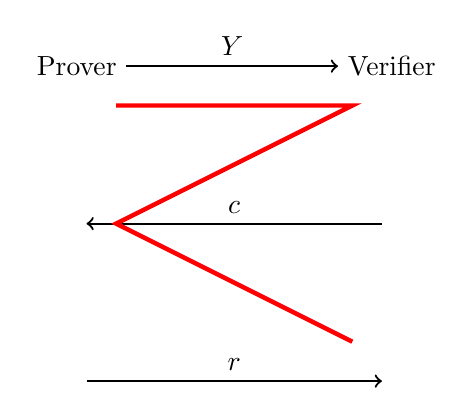
\begin{tikzpicture}
					\node (P1) at (0,0) {Prover};
					\node (V1) at (4,0) {Verifier};
					\node (P2) at (0,-2) {};
					\node (V2) at (4,-2) {};
					\node (P3) at (0,-4) {};
					\node (V3) at (4,-4) {};

					\draw[->, thick] (P1) -- node[above] {$Y$} (V1);
					\draw[->, thick] (V2) -- node[above] {$c$} (P2);
					\draw[->, thick] (P3) -- node[above] {$r$} (V3);

					\draw[red, ultra thick] (0.5,-0.5) -- (3.5,-0.5) -- (0.5,-2) -- (3.5,-3.5);
				\end{tikzpicture}
			\end{center}
		\end{column}
		\begin{column}{0.5\textwidth}
			\textbf{The Greek letter $\Sigma$ (Sigma)}
			\begin{itemize}
				\item Three message flows
				\item Alternating direction
				\item Forms a ``zigzag'' pattern
				\item Hence: Sigma protocols!
			\end{itemize}
			\vspace{0.5em}
			\begin{alertblock}{Always this pattern}
				\begin{enumerate}
					\item Prover $\rightarrow$ Verifier: Commitment
					\item Verifier $\rightarrow$ Prover: Challenge
					\item Prover $\rightarrow$ Verifier: Response
				\end{enumerate}
			\end{alertblock}
		\end{column}
	\end{columns}
\end{frame}

\begin{frame}{Formal definition of Sigma protocols}
	\begin{block}{Definition: Sigma Protocol}
		A sigma protocol consists of the following parameters:
		\begin{itemize}
			\item \textbf{Commit}: A randomized algorithm that takes instance $X$ and witness $W$ as input, outputs commitment $Y$ and state $\sigma$
			\item $\mathcal{C}$: A set of verifier challenges
			\item \textbf{Respond}: A deterministic algorithm that takes state $\sigma$ and challenge $c \in \mathcal{C}$ as input, outputs response $r$
			\item \textbf{Check}: A deterministic algorithm that takes transcript $(X, Y, c, r)$ as input, outputs true/false
		\end{itemize}
	\end{block}
\end{frame}

\begin{frame}{Example: Schnorr as Sigma protocols}
	\begin{columns}[c]
		\begin{column}{0.5\textwidth}
			\textbf{Instance and Witness:}
			\begin{itemize}
				\item Instance: $X = A = g^a$
				\item Witness: $W = a$
				\item Relation: $g^W = X$
			\end{itemize}
			\vspace{0.5em}
			\textbf{The Algorithms:}
			\begin{itemize}
				\item \textbf{Commit}$(A, a)$:
				      \begin{itemize}
					      \item $y \twoheadleftarrow \mathbb{Z}_n$
					      \item $Y = g^y$
					      \item Return $(Y, \sigma = y)$
				      \end{itemize}
			\end{itemize}
		\end{column}
		\begin{column}{0.5\textwidth}
			\begin{itemize}
				\item $\mathcal{C} = \mathbb{Z}_n$ (all possible challenges)
				\item \textbf{Respond}$(\sigma = y, c)$:
				      \begin{itemize}
					      \item Return $r = y + ca \bmod n$
				      \end{itemize}
				\item \textbf{Check}$(A, Y, c, r)$:
				      \begin{itemize}
					      \item Return $(g^r = Y \cdot A^c)$
				      \end{itemize}
			\end{itemize}
			\vspace{0.5em}
			\begin{exampleblock}{Fits the framework!}
				Schnorr is just one example of a Sigma protocol
			\end{exampleblock}
		\end{column}
	\end{columns}
\end{frame}

\begin{frame}{Example: proving knowledge of a representation}
	\begin{columns}[c]
		\begin{column}{0.5\textwidth}
			\textbf{The problem:}
			\begin{itemize}
				\item Given: $X = g^a h^b$
				\item Prove: ``I know $(a, b)$''
				\item Without revealing $(a, b)$!
			\end{itemize}
			\vspace{0.5em}
			\textbf{Why is this useful?}
			\begin{itemize}
				\item Pedersen commitments
				\item Mix networks
				\item Electronic voting
			\end{itemize}
		\end{column}
		\begin{column}{0.5\textwidth}
			\textbf{The Sigma protocol:}
			\begin{itemize}
				\item \textbf{Commit}:
				      \begin{itemize}
					      \item Pick random $r, s$
					      \item $Y = g^r h^s$
					      \item State: $\sigma = (r, s)$
				      \end{itemize}
				\item \textbf{Respond}:
				      \begin{itemize}
					      \item $u = r + ca$
					      \item $v = s + cb$
					      \item Return $(u, v)$
				      \end{itemize}
				\item \textbf{Check}:
				      \begin{itemize}
					      \item $g^u h^v \overset{?}{=} Y \cdot X^c$
				      \end{itemize}
			\end{itemize}
		\end{column}
	\end{columns}
\end{frame}

\begin{frame}{The power of Sigma protocols}
	\begin{center}
		\textbf{Sigma protocols can prove almost any statement!}
	\end{center}
	\vspace{0.5em}
	\begin{columns}[c]
		\begin{column}{0.5\textwidth}
			\textbf{Graph Problems:}
			\begin{itemize}
				\item ``I know a 3-coloring of this graph''
				\item ``I know a Hamiltonian cycle''
				\item ``I know an isomorphism between graphs''
			\end{itemize}
			\vspace{0.5em}
			\textbf{Number Theory:}
			\begin{itemize}
				\item ``I know the square root of $X$ mod $N$''
				\item ``I know the factorization of $N$''
			\end{itemize}
		\end{column}
		\begin{column}{0.5\textwidth}
			\textbf{Cryptographic Statements:}
			\begin{itemize}
				\item ``This ciphertext encrypts 0 or 1''
				\item ``These ciphertexts encrypt the same value''
				\item ``I shuffled these ciphertexts correctly''
			\end{itemize}
			\vspace{0.5em}
			\begin{alertblock}{Universal result}
				Any NP statement has a Sigma protocol!
			\end{alertblock}
		\end{column}
	\end{columns}
\end{frame}

\section{Proving AND, OR}

\begin{frame}{Composing Sigma protocols: AND, OR}
	\begin{columns}[c]
		\begin{column}{0.5\textwidth}
			\textbf{Proving AND statements:}
			\begin{itemize}
				\item ``I know $a$ AND I know $b$''
				\item Run both protocols in parallel
				\item Use the same challenge for both
				\item Verifier checks both conditions
			\end{itemize}
			\vspace{0.5em}
			\textbf{Example:}
			\begin{itemize}
				\item Prove: ``I know $x$ such that $g^x = A$ AND $h^x = B$''
				\item Shows same secret used in multiple places
			\end{itemize}
		\end{column}
		\begin{column}{0.5\textwidth}
			\textbf{Proving OR statements:}
			\begin{itemize}
				\item ``I know $a$ OR I know $b$''
				\item More complex: need to hide which one
				\item Simulate one proof, execute the other
				\item Verifier can't tell which is real!
			\end{itemize}
			\vspace{0.5em}
			\textbf{Example:}
			\begin{itemize}
				\item Prove: ``I know the key for account A OR account B''
				\item Privacy-preserving authentication
			\end{itemize}
		\end{column}
	\end{columns}
\end{frame}

\begin{frame}{Special Soundness: why Sigma protocols are secure}
	\begin{itemize}
		\item TODO
	\end{itemize}
\end{frame}

\begin{frame}{From Interactive to Non-Interactive}
	\begin{columns}[c]
		\begin{column}{0.5\textwidth}
			\textbf{The limitation:}
			\begin{itemize}
				\item Sigma protocols require interaction
				\item Verifier must be online
				\item Can't create transferable proofs
				\item Can't post proofs publicly
			\end{itemize}
			\textbf{The goal:}
			\begin{itemize}
				\item Create a proof once
				\item Anyone can verify it later
				\item No interaction needed
			\end{itemize}
		\end{column}
		\begin{column}{0.5\textwidth}
			\begin{block}{Coming next...}
				The Fiat-Shamir transform:
				\begin{itemize}
					\item Replace verifier with a hash function
					\item Challenge = $H(X, Y)$
					\item Prover can't cheat the hash!
					\item Creates non-interactive proofs
				\end{itemize}
			\end{block}
		\end{column}
	\end{columns}
\end{frame}

\incompleteslideswarning

\section{Non-Interactive Zero-Knowledge Proofs}

\incompleteslideswarning

\incompleteslideswarning

\section{Zero-Knowledge Virtual Machines}

\incompleteslideswarning

\incompleteslideswarning

\begin{frame}[plain]
	\titlepage
\end{frame}
\end{document}
